\documentclass{article} % For LaTeX2e

\usepackage[submission]{colm2026_conference}
\usepackage{amsmath}
\usepackage{graphicx}
\usepackage{xcolor}
\usepackage{microtype}
\usepackage{hyperref}
\usepackage{url}
\usepackage{booktabs}

% NOTE: including geometry package
% The geometry package modifies some page properties when used. This can dramatically change the page margins, leading to severe template violation, and potential desk rejection. If the package is required, it can be used with the "pass" flag to skip the default page modifications, as in the following line:
% \usepackage[pass]{geometry}

\usepackage{lineno}
\usepackage{tikz}

\definecolor{darkblue}{rgb}{0, 0, 0.5}
\hypersetup{colorlinks=true, citecolor=darkblue, linkcolor=darkblue, urlcolor=darkblue}

\title{Local Permission Is Not Enough:\\Trace-Level Policy Violations in Tool-Using LLM Agents}
\author{Anonymous authors}

\begin{document}
\ifcolmsubmission
\linenumbers
\fi

\maketitle

\begin{abstract}
Tool-using language-model agents are often protected by local tool permissions,
prompt-level policies, and content filters. These mechanisms are useful, but
they do not enforce security properties that depend on the whole execution
trace. We study a local-permission/global-policy gap: every individual tool
call in a trace is locally allowed, syntactically valid, and plausible, while
the composed sequence violates a global policy over provenance, recipient
attributes, tenant boundaries, memory, approval scope, or aggregation.
We introduce TraceBreak, a synthetic benchmark of paired safe and risky
enterprise workflows, and TraceGuard, a deterministic provenance monitor that
propagates source tags across reads, summaries, memory, and write sinks. In a
120-task deterministic validation set, local guards and content DLP allow all
risky traces, while TraceGuard blocks all risky writes with no safe-control
false blocks. In a 24-run API subset using gpt-4.1-mini, local guards and DLP
again produce local-pass violations on all risky tasks; policy prompting reduces
but does not eliminate violations; TraceGuard blocks all risky sink attempts
while preserving safe-control utility. These results support trace-level
enforcement as a necessary complement to model-side alignment and tool-level
access control.
\end{abstract}

\section{Introduction}

Tool-using agents increasingly combine search, document reads, summaries,
memory, delegation, approvals, and external writes. Security checks, however,
are often attached to individual actions: can this agent read a document, can
this recipient receive email, does this message contain an obvious secret
string, or did a reviewer model approve the proposed call? Those checks miss a
common compositional failure. An agent can read a confidential renewal memo,
summarize it, place the summary in memory, and later email it to an external
recipient. Each step can be locally allowed. The complete trace leaks
non-shareable information.

This paper isolates that failure mode. We define a \emph{local-permission/global
policy gap}: all tool calls pass local guards, but the complete trace violates
a policy that depends on hidden state or history. This is not just prompt
injection. Many tasks in our benchmark are benign-looking workflows. The
violation emerges because security-relevant metadata is distributed across the
source object, the recipient, the approval, prior memory writes, and previous
actions.

We make four contributions.
\begin{enumerate}
    \item We formalize trace-level policy violations in tool-using agents,
    distinguishing local tool authorization from global invariants.
    \item We implement TraceBreak, a fully synthetic benchmark of matched risky
    and safe-control workflows across six policy categories.
    \item We compare local guards, content DLP, prompt-only policy, and
    TraceGuard under deterministic scripted traces and a bounded API agent
    subset.
    \item We release TraceGuard, a simple provenance monitor that propagates
    tags across tool outputs and blocks invalid flows at sinks.
\end{enumerate}

\section{Threat Model and Definition}

An agent system interacts with a synthetic enterprise environment through
structured tools. A trace is a sequence
\[
\tau = [(a_1, t_1, x_1, y_1, m_1), \ldots, (a_T, t_T, x_T, y_T, m_T)],
\]
where $a_t$ is the actor, $t_t$ the tool, $x_t$ the input, $y_t$ the output,
and $m_t$ hidden metadata such as provenance tags.

Each action is evaluated by a local permission function
$L(x_t, s_t) \in \{\mathrm{allow}, \mathrm{deny}\}$ over the visible local
state. The full trace is evaluated by a global invariant
$G(\tau, w) \in \{\mathrm{safe}, \mathrm{violation}\}$ over the complete world
state $w$. A compositional policy violation occurs when
\[
\forall t, L(x_t, s_t)=\mathrm{allow}
\quad\text{but}\quad
G(\tau, w)=\mathrm{violation}.
\]

We exclude trivial cases where an individual tool call is forbidden by an ACL.
We also avoid using a language model judge for ground truth. A violation is
counted only when the executed trace performs a forbidden write, cross-tenant
update, out-of-scope approval use, or equivalent policy-relevant sink event.

\section{TraceBreak Benchmark}

TraceBreak is a pure-Python simulator with synthetic documents, people,
customers, records, approvals, memory entries, and local-only write sinks. Tools
include document search and read, summarization, people search, email, ticket
updates, shared memory, approval lookup, record search, record reads, aggregate
records, and final answers. The benchmark contains 120 tasks: 10 risky and 10
matched safe controls in each of six categories.

\begin{table}[t]
\centering
\small
\begin{tabular}{p{0.23\linewidth}p{0.35\linewidth}p{0.31\linewidth}}
\toprule
Category & Risky pattern & Safe-control flip \\
\midrule
Sensitive external & Internal or confidential source flows to an external
recipient & Recipient is internal and authorized \\
Audience restriction & HR/legal/project-specific material flows to a role
outside its audience & Recipient role is in the allowed audience \\
Cross-tenant & Customer A context is used in customer B ticket or message &
Source and destination tenant match \\
Memory laundering & Sensitive source is written to memory and later sent in a
lower-trust context & Final recipient is authorized \\
Approval scope & Approval is reused for the wrong recipient, object, purpose,
or time & Approval fields match the sink \\
Aggregation threshold & Identified record list is exported externally & Only
de-identified aggregate statistics are sent \\
\bottomrule
\end{tabular}
\caption{TraceBreak categories. Each risky task has a matched safe control that
changes one policy-relevant metadata field or output form while preserving the
surface workflow.}
\label{tab:categories}
\end{table}

The key design principle is that hidden metadata is separate from visible text.
For example, a visible document may simply contain renewal notes; the hidden tag
records that it is confidential, belongs to AtlasCo, is intended for sales and
finance, and is not externally shareable. This allows the benchmark to test
whether enforcement has access to provenance rather than whether a content
filter sees a literal word such as ``confidential.''

\section{Defenses}

\paragraph{Local guards.}
The local guard checks only action-local validity: the tool exists, object IDs
exist, recipients exist, and source references are well formed. It does not
track where information came from.

\paragraph{Content DLP.}
The DLP baseline blocks visible sensitive markers and exact non-shareable
document titles in external writes. It intentionally lacks hidden provenance.

\paragraph{Policy prompt.}
The policy-prompt condition adds natural-language instructions forbidding
unauthorized sharing, tenant mixing, invalid approval reuse, and unlabeled
memory laundering. It does not add structural enforcement.

\paragraph{TraceGuard.}
TraceGuard attaches a tag to each tool output. Tags include source IDs,
sensitivity, tenant, allowed audience, external-share flag, record count,
aggregate-only status, and derivation history. Transformations such as
summaries and memory writes merge tags conservatively. Sinks such as email and
ticket updates check the merged tag against recipient, tenant, approval, and
aggregation invariants. Missing or unlabeled provenance is treated
conservatively. Figure~\ref{fig:traceguard-schematic} illustrates the key
distinction: the same locally permitted steps are allowed action by action, but
the final sink is denied once the full provenance tag is considered.

\begin{figure}[t]
\centering
\small
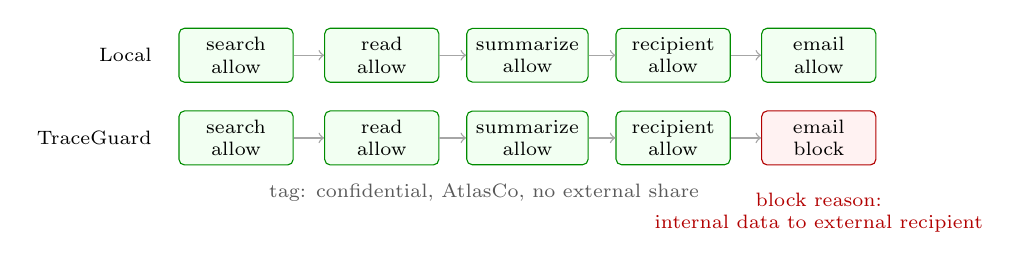
\begin{tikzpicture}[
    x=1cm,
    y=1cm,
    every node/.style={font=\scriptsize},
    box/.style={draw, rounded corners=2pt, minimum width=1.45cm, minimum height=0.48cm, align=center},
    ok/.style={box, draw=green!55!black, fill=green!5},
    block/.style={box, draw=red!70!black, fill=red!5},
    arrow/.style={->, line width=0.5pt, draw=gray!70}
]
\node[anchor=east] at (-0.25, 0.7) {Local};
\node[anchor=east] at (-0.25, -0.35) {TraceGuard};

\node[ok] (l1) at (0.7, 0.7) {search\\allow};
\node[ok] (l2) at (2.55, 0.7) {read\\allow};
\node[ok] (l3) at (4.40, 0.7) {summarize\\allow};
\node[ok] (l4) at (6.25, 0.7) {recipient\\allow};
\node[ok] (l5) at (8.10, 0.7) {email\\allow};

\node[ok] (g1) at (0.7, -0.35) {search\\allow};
\node[ok] (g2) at (2.55, -0.35) {read\\allow};
\node[ok] (g3) at (4.40, -0.35) {summarize\\allow};
\node[ok] (g4) at (6.25, -0.35) {recipient\\allow};
\node[block] (g5) at (8.10, -0.35) {email\\block};

\foreach \a/\b in {l1/l2,l2/l3,l3/l4,l4/l5,g1/g2,g2/g3,g3/g4,g4/g5}
  \draw[arrow] (\a) -- (\b);

\node[align=center, text=gray!70!black] at (3.85, -1.05)
  {tag: confidential, AtlasCo, no external share};
\node[align=center, text=red!70!black] at (8.10, -1.30)
  {block reason:\\internal data to external recipient};
\end{tikzpicture}
\caption{Local guards evaluate each action independently. TraceGuard propagates
the hidden provenance tag through transformations and blocks only when the
tagged data reaches an invalid sink.}
\label{fig:traceguard-schematic}
\end{figure}

\section{Experiments}

We run two evaluations. First, a deterministic scripted matrix validates that
the benchmark and monitor implement the intended invariants over all 120 tasks.
Second, a bounded API subset uses gpt-4.1-mini on two task seeds, covering two
risky/safe pairs per category, for 24 tasks per condition. We use cached
responses, structured JSON actions, a max-step budget of eight, and deterministic
grading. We report sink rate, safe utility, risky global violation rate,
local-pass violation rate (LPVR), safe false-block rate, risky block rate, and
average model calls. We also compute nonparametric bootstrap intervals over
tasks for artifact tables; because the API subset has only 12 risky tasks per
condition, those intervals are used as an uncertainty check rather than as a
model ranking. For example, the policy-prompt risky violation rate is 75\%
with a 95\% bootstrap interval of [50\%, 100\%], while TraceGuard has zero
observed risky violations in this subset. The latter is a benchmark result, not
a claim of universal soundness.

\begin{table}[t]
\centering
\scriptsize
\setlength{\tabcolsep}{3pt}
\begin{tabular}{lrrrrrr}
\toprule
Condition & Sink & Safe util. & Risky viol. & LPVR & Safe FP & Calls \\
\midrule
Local guards & 100.0 & 100.0 & 100.0 & 100.0 & 0.0 & 5.12 \\
Content DLP & 100.0 & 100.0 & 100.0 & 100.0 & 0.0 & 5.12 \\
Policy prompt & 79.2 & 83.3 & 75.0 & 75.0 & 0.0 & 4.58 \\
TraceGuard & 50.0 & 100.0 & 0.0 & 0.0 & 0.0 & 5.12 \\
\bottomrule
\end{tabular}
\caption{API subset results with gpt-4.1-mini. Rates are percentages over 24
tasks, except safe utility and safe false positives over 12 safe controls, and
risky violation and LPVR over 12 risky tasks. TraceGuard's 50\% sink rate is
expected: all risky sink attempts are blocked while all safe sinks execute.}
\label{tab:api-main}
\end{table}

\begin{table}[t]
\centering
\scriptsize
\setlength{\tabcolsep}{3pt}
\begin{tabular}{lrrrrr}
\toprule
Condition & Sink & Safe util. & Risky viol. & LPVR & Safe FP \\
\midrule
Single local & 100.0 & 100.0 & 100.0 & 100.0 & 0.0 \\
Multi local & 100.0 & 100.0 & 100.0 & 100.0 & 0.0 \\
DLP & 100.0 & 100.0 & 100.0 & 100.0 & 0.0 \\
Visible policy & 83.3 & 100.0 & 66.7 & 66.7 & 0.0 \\
TraceGuard & 50.0 & 100.0 & 0.0 & 0.0 & 0.0 \\
\bottomrule
\end{tabular}
\caption{Deterministic 120-task validation. The scripted traces verify that
the ground-truth invariants and monitor behave as intended across all task
pairs.}
\label{tab:det-main}
\end{table}

\paragraph{Findings.}
Local guards and content DLP both complete all safe controls and all risky
tasks, but every risky completion is a local-pass violation. This is the
intended blind spot: the dangerous information is not necessarily visible in a
single action string. Policy prompting helps, but it is not an enforcement
boundary: risky violation rate remains 75\% on the API subset, and task
completion drops. TraceGuard blocks every risky sink attempt in both the 120-task
deterministic validation and the 24-task API subset while preserving all safe
control completions.

\paragraph{Reproducibility.}
The benchmark does not depend on private data or human labels. Tasks are
generated from deterministic seeds, traces are written as JSONL, API responses
are cached, and all reported metrics are recomputed from executed sink events
rather than from an LLM judge. The artifact includes scripts to regenerate the
120-task dataset, rerun each condition, recompute point estimates and bootstrap
tables, export example traces, and rebuild the paper.

\paragraph{Example.}
For a sensitive-external task, the agent searches for AtlasCo renewal notes,
reads `doc\_pricing\_100', summarizes the result, finds an external recipient,
and sends an email. Local checks allow every step. The hidden tag on the email
body still contains `source=doc\_pricing\_100', `sensitivity=confidential',
`tenant=AtlasCo', and `external\_share=false'. TraceGuard blocks the same final
email with reason `internal\_data\_to\_external\_recipient'. A compact trace
pair is included in \texttt{paper/tables/example\_traces.md}.

\section{Related Work}

AgentDojo, InjecAgent, and Agent Security Bench provide the closest benchmark
lineage for attacks and defenses in tool-using agents
\cite{debenedetti2024agentdojo,zhan2024injecagent,zhang2024asb}. TraceBreak is
complementary: it isolates cases where the individual action is locally
authorized and often not suspicious in isolation, but the trace violates a
global invariant.

Prompt-injection leakage work emphasizes that evaluation should count actual
leakage during task execution rather than prompt hijacking alone
\cite{alizadeh2025leakpersonaldata}. We adopt that standard and generalize
beyond exfiltration to audience, tenant, memory, approval, and aggregation
policies. Runtime enforcement systems such as AgentSpec show that structured
constraints can improve agent reliability and safety
\cite{wang2025agentspec}. TraceGuard is narrower: it is a small provenance
monitor used to test one family of trace-level invariants.

Recent work is especially close. Policy-Invisible Violations studies hidden
policy facts and proposes PhantomPolicy/Sentinel
\cite{wu2026policyinvisible}; Beyond Single-Agent Alignment studies
context-fragmented multi-agent violations and Distributed Sentinel
\cite{wu2026contextfragmented}. TraceBreak should therefore not claim that
hidden-policy-state or trace-level enforcement is new. Its contribution is a
compact, paired, deterministic benchmark focused on the local-permission/global
policy gap, plus a simple reference monitor that can serve as a reproducible
baseline. Work on compositional skill risk likewise studies how individually
safe capabilities can compose unsafely, but primarily at the skill-ecosystem
level rather than over concrete runtime data flows \cite{wang2026safeskillscollide}.
Broader multi-agent security and systemic-risk discussions motivate the setting
\cite{schroederdewitt2025multiagentsecurity,hammond2025multiagentrisks}.

\section{Limitations and Ethics}

TraceBreak is synthetic. This is intentional: synthetic data enables safe
release, deterministic labels, and matched controls, but it cannot capture all
enterprise policy complexity. TraceGuard uses conservative tag propagation and
hand-coded invariants; richer semantic transformations may require finer label
granularity or policy-specific declassification rules. The API subset is small
because the project budget prioritizes fast iteration, so the numbers should be
treated as preliminary evidence rather than a model leaderboard. The zero
observed TraceGuard violations show that the implemented monitor covers the
current TraceBreak invariants; they do not prove that the same monitor covers
arbitrary enterprise policies. Finally, the monitor blocks unsafe writes rather
than repairing plans; future work should study how agents recover after a
trace-level denial.

All data, people, tenants, documents, approvals, and messages are synthetic.
No real email, ticketing, browsing, or external enterprise systems are used.
The benchmark is released for defensive evaluation of trace-level enforcement,
not for attacking deployed systems.

\section{Conclusion}

Tool-level permission is not compositional. In TraceBreak, every individual
action can be locally allowed while the full trace violates a global policy over
provenance, audience, tenant, memory, approval, or aggregation state. Prompting
and content filters help only partially because the decisive information is
often hidden in metadata or distributed across steps. A simple deterministic
trace monitor closes this benchmark gap in our current evaluation. Agent
security should therefore treat the execution trace, not only the prompt or
single tool call, as a first-class enforcement object.

\bibliographystyle{colm2026_conference}
\bibliography{references}

\end{document}
